%!TEX root = syntheyes15.tex

\section{Our dynamic eye-region model}

\begin{figure*}
    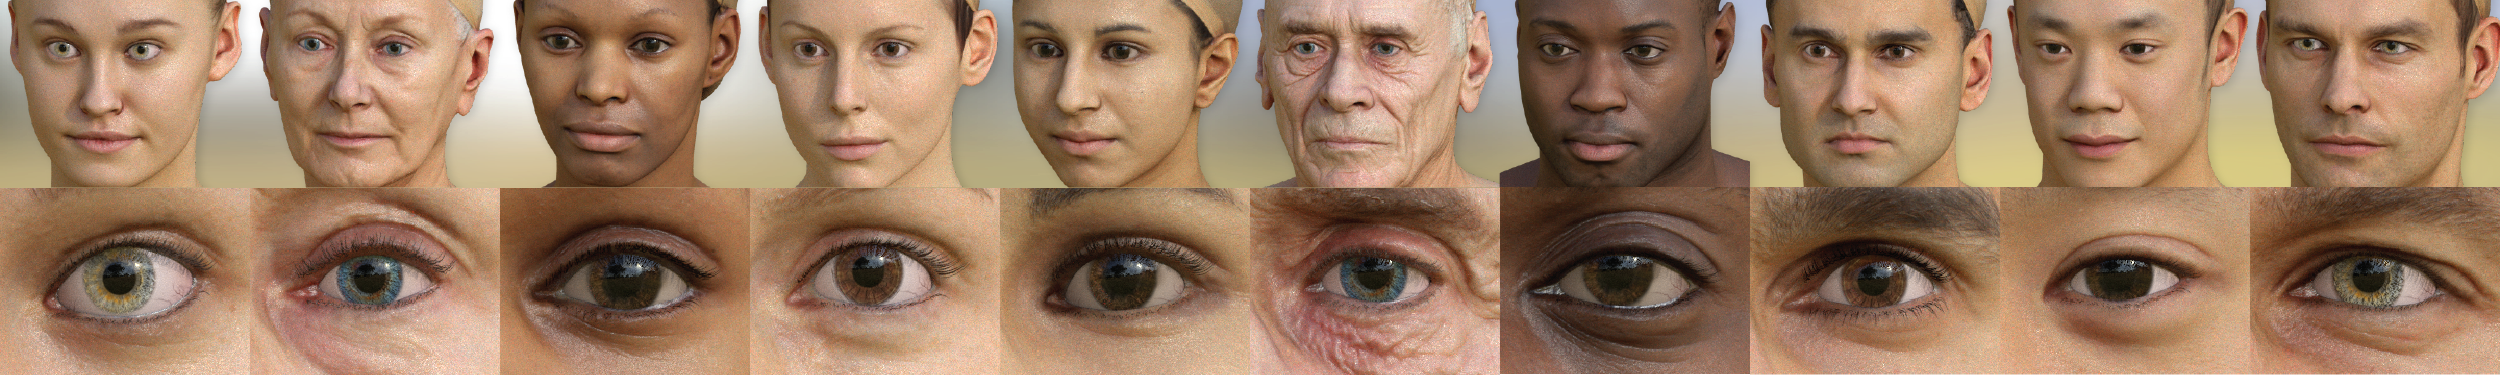
\includegraphics[width=\textwidth]{model_suite}
    \caption{Set of head models and corresponding close-ups of the eye regions used in our method. The set includes 10 different head models of both genders that cover a range of ethnicities and ages.}
    \label{fig:model_suite}
\end{figure*}

In this section we first present our anatomically inspired CG eyeball model, and then explain our novel procedure for preparing a suite of 3D head scans for dynamic photorealistic labelled data generation.

% \cite{MIL-STD-1472G} -- cite for range of eye rotation.

\subsection{Reduced eyeball model}
\label{subsec:eyeball_model}

\begin{figure}
    \centering
    \begin{subfigure}[t]{0.33\columnwidth}
        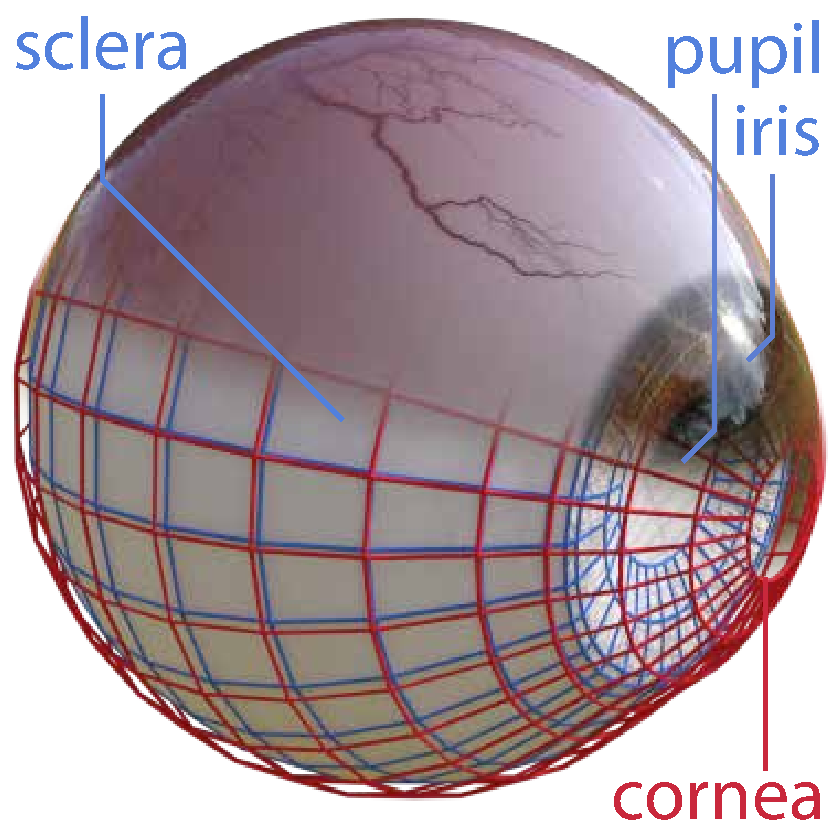
\includegraphics[width=\textwidth]{eye_model}
        \caption{3D eye model}
        \label{fig:3d_eye_model}
    \end{subfigure}%
    \hfill
    \begin{subfigure}[t]{0.65\columnwidth}
        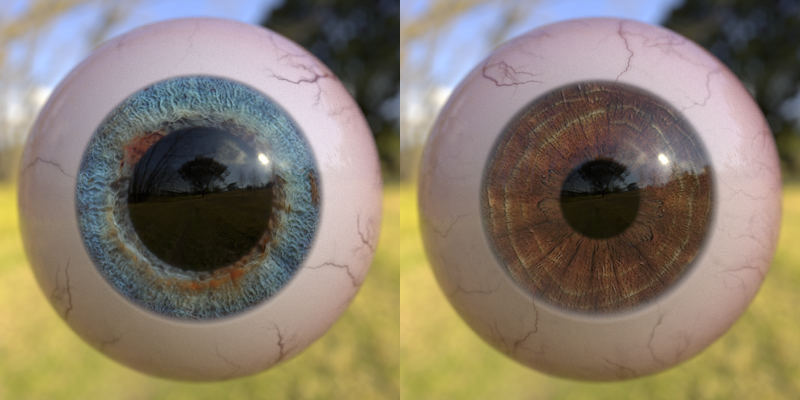
\includegraphics[width=\textwidth]{eye_examples}
        \caption{Pupil dilation and iris color variation}
    \end{subfigure}
    \caption{Our realistic eye model is capable of expressing degrees of variability seen in real life.}
    \label{fig:eye_model}
\end{figure}

Eyeballs are complex organs comprised of multiple layers of tissue, each with different reflectance properties and levels of transparency. Fortunately, as realistic eyes are so important for many areas of CG, there is already a large body of previous work on modelling and rendering eyes \commentE{cite}.

% It is important to accurately model reflections and refractions in the eye as they can lead to specular highlights -- these common eye-region image features are often used by eye-tracking algorithms, or can confound approaches that are not robust.

As shown in \autoref{fig:3d_eye_model}, our eye model consists of two parts.
%
The outer part (red wireframe) approximates the eye's overall shape with two spheres ($r_1\!=\!12\textrm{mm}, r_2\!=\!8\textrm{mm}$ \cite{ruhland2014look}), the latter representing the corneal bulge. To avoid a discontinuous seam between spheres, the meshes were joined and then smoothed. It is transparent, refractive ($n\!=\!1.376$), and partially reflective. The eye's bumpy surface variation is modelled by a displacement map generated with noise functions.
%
The inner part (blue wireframe) is a flattened sphere with Lambertian material. The planar end represents the iris and pupil, and the rest represents the sclera -- the white of the eye.
%
There is a $0.5\textrm{mm}$ gap between the outer and inner parts which accounts for the thickness of the cornea. \commentE{compare with recent Disney work}

Eyes exhibit variations in both shape (pupillary dilation) and texture (iris color and scleral veins). To model shape variation we use \emph{shape keys} -- a CG animation technique where different versions of a mesh are stored, modified, and interpolated between \cite{orvalho2012facial}. \commentE{more on shape keys} We have shape keys representing dilated and constricted pupils, as well as large and small irises to account for a small amount ($10\%$) of variation in iris size.

We vary the appearance of the eye by compositing textures in three separate layers:
\begin{inparaenum}[\itshape i\upshape)]
\item a \emph{sclera} layer representing the tint of the sclera (white, pink, or yellow);
\item an \emph{iris} layer with four photo-textures of different colored irises (amber, blue, brown, grey); and
\item a \emph{veins} layer which varies between blood-shot and clear
\end{inparaenum}. We matched the sclera tint to each separate face model, but uniformably randomly varied iris color. Previous research on iris-synthesis \commentE{cite} would have allowed continually different iris textures, but we decided this added complexity would not make a worthwhile improvement in overall appearance variation, especially when rendered at lower resolutions.

\subsection{3D head scan acquisition}

\begin{figure*}
    \centering
    \begin{subfigure}[t]{0.195\textwidth}
        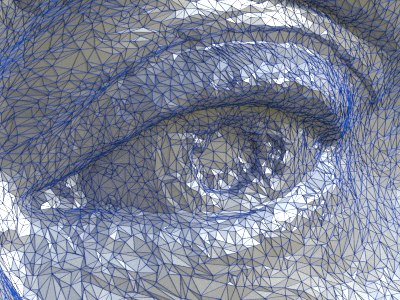
\includegraphics[width=\textwidth]{process_f02_01}
        \caption{Original 3D head scan data: 1.4 million polys}
        \label{fig:process_original_scan}
    \end{subfigure}
    \hfill
    \begin{subfigure}[t]{0.195\textwidth}
        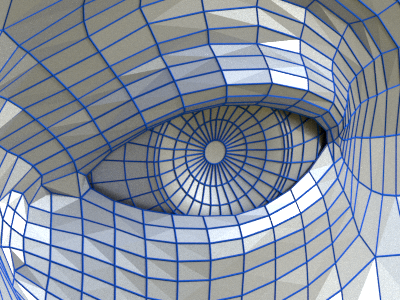
\includegraphics[width=\textwidth]{process_f02_02}
        \caption{Retopologized head model: 9 thousand polys}
        \label{fig:process_retopo}
    \end{subfigure}
    \hfill
    \begin{subfigure}[t]{0.195\textwidth}
        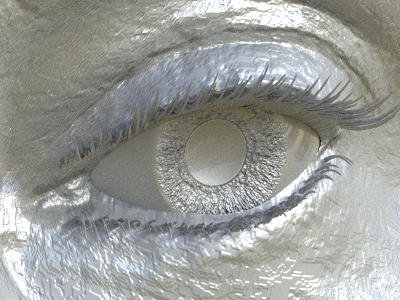
\includegraphics[width=\textwidth]{process_f02_03}
        \caption{Surface detail is stored in displacement maps}
        \label{fig:process_displaced_subdiv}
    \end{subfigure}
    \hfill
    \begin{subfigure}[t]{0.195\textwidth}
        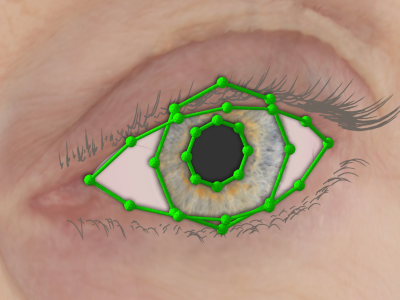
\includegraphics[width=\textwidth]{process_f02_04}
        \caption{3D iris and eyelid landmarks are annotated}
    \end{subfigure}
    \hfill
    \begin{subfigure}[t]{0.195\textwidth}
        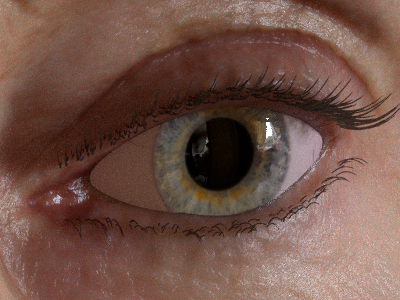
\includegraphics[width=\textwidth]{process_f02_05}
        \caption{The final render}
    \end{subfigure}
    \caption{Model preparation process}
    \label{fig:process}
\end{figure*}

Photogrammetry is becoming a popular ...

We start with high quality production-level scans purchased from a photogrammetry studio's online store.

\subsection{Eye-region geometry preparation}

As can be seen in \autoref{fig:process_original_scan}, the cornea has been incorrectly reconstructed in the head scan. This is because transparent surfaces are not directly visible, so cannot be reconstructed in the same way as diffuse surfaces like skin. Recent work uses a hybrid reconstruction method to reconstruct the corneal surface seprately, but requires additional hardware \cite{berard2014highquality} -- this level of detail was deemed unneccesary for our purposes. We want to render eye-region images representing a wide range of eye-gaze directions, so we need to be able to pose the eyeball separately from the face geometry. We therefore remove the scanned eyeball from the mesh using boolean operations, and place our own eyeball approximation (\autoref{subsec:eyeball_model}) in its place.

While the original head scan geometry is suitable for being rendered as a static model, its topology cannot easily represent dynamic changes in eye-region shape. Vertical saccades are always accompanied by eyelid motion \cite{liversedge2011oxford}, so we need to be able to pose the eyelids according to the gaze vector. When preparing a mesh for facial animation, edge loops should flow along and around the natural contours of facial muscles. This leads to a more efficient (lower-resolution) geometric representation of the face, and more realistic animation as mesh deformation mathes that of actual muscles.

We therefore \emph{retopologize} the face geometry into a more optimal form using a commercial semi-automatic system \cite{ZRemesher}. \commentE{Reference some other options, e.g automatic methods in research} As can be seen in \autoref{fig:process_retopo}, edge loops now follow the \emph{Orbicularis Oculi} muscle, allowing for realistic eye-region deformations. This retopologized low-poly mesh lacks the detail of the original scan (e.g. the crease above the eye), and has visible sharp edges. We therefore use it as the control mesh for a displaced subdivision surface \cite{lee2000displaced}, with displacement map computed from the scanned geometry. As can be seen in \autoref{fig:process_displaced_subdiv}, skin surface detail like wrinkles and creases is  restored.

Although they are two seperate organs, there is normally no visible gap between eyeball and skin. However, as a consequence of removing the eyeball from the original scan, the retopologized mesh will not necessarily meet the geometry of our eyeball model (\autoref{fig:process_retopo}). To compensate, the face mesh's eyelid vertices are displaced along their normals to their respective closest positions on the eyeball geometry (\autoref{fig:process_displaced_subdiv}). This automatic operation ensures the models are joined, even after changes in pose \cite{Shrinkwrap}.

\subsection{Eyelashes}

Eyelashes are short curved hairs that grow from the outer edges of the eyelids. These can occlude parts of the eye and affect eye-tracking algorithms, so should be simulated. We follow the approach of \citet{swirski2014rendering}, and model them using directed hair particle effects. The hair particles are generated from a smoothed control surface below the eyelid edges and directed away from the face. To make them curl, the eyelash particles experience a slight amount of gravity during growth (negative gravity for the upper eyelash).

\subsection{Eyelid motion}

Create face, eyelash, and landmark blend shapes for eyelids looking up and down.

\begin{figure}
    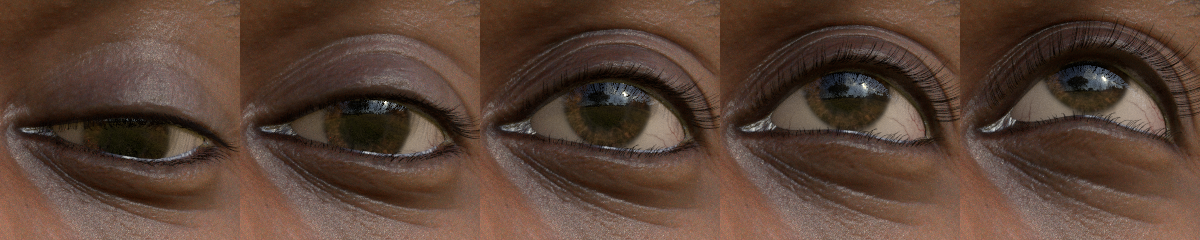
\includegraphics[width=\columnwidth]{eyelid_motion.png}
    \caption{Eyelids are posed using blend shapes linked to the gaze vector. Note how we use wrinkle-maps to simulate the folding of the skin above and below the eye.}
\end{figure}